\chapter{Test}

I dette afsnit vil vi forklare, hvordan vi har lavet test af vores software.
Vi har blandt andet gjort brug af unit tests og test cases.

\section{Unit test}

For at softwaren bag holder en vis kvalitet, er der udført en generel unit test på klasserne i spillet.
Denne unit test indebærer simple test af alle metoder i klasserne.
Derudover er lavet to udvidede test.
\\
Den ene, tester om terningen er fair, med 60000 kast og en fejlmargen på 400 slag pr. side af terningen.
Den anden, kigger på, om sandsynlighederne for de respektive summe, ved to terninger er sandsynligt korrekte.
Dette gøres også ved 60000 kast, med 2 terninger, for derefter at beregne sandsynligheden, for den respektive sum, samt det faktiske resultat.
Nedenfor ses det udsnit af testen, som ordner denne beregning.
\\

\begin{lstlisting}
double oneRollPercent = (double) 100 / numberOfRolls;
    
double totalPercentage = 0;
double failureRate = 0.75;
for (int i = numberOfDies; i < rolls.length; i++) {
    double percentage = (double) rolls[i] * oneRollPercent;
    int posibilities = this.numPossibilities(numberOfDies, i);
    double expectedPercentage = posibilities * (100.0 / 36.0);

    totalPercentage += percentage;
}
\end{lstlisting}
\newpage
\section{Testcases}
Herunder er en række testcases, som er blevet udarbejdet ud fra vores krav og mål.
Alle test er blevet testet i IntelliJ.
\\\\Testcase 1 handler om, hvorvidt programmet tager korrekt imod Strings, når den beder om navne, og hvorvidt det bliver gemt.
Det ville blive kaotisk, hvis der var blevet sat et navn til f.eks. Player1, og programmet så senere omtaler Player1 som Player1 og ikke det pågældende navn.

\begin{figure}[h]
    \begin{center}
        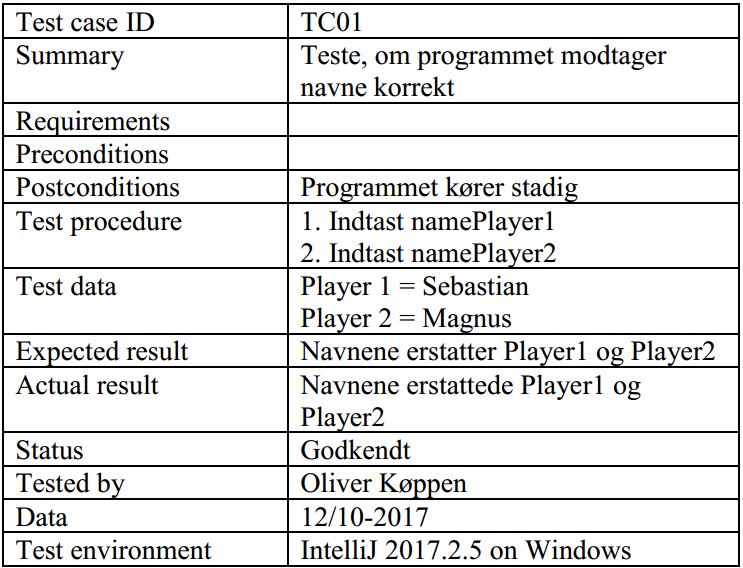
\includegraphics[width=10cm]{graphics/TC01}
    \end{center}
\end{figure}

Testcase 2 handler om, hvorvidt programmet kan tage imod to ens terninger og Testcase 2 handler om, hvorvidt programmet kan tage imod to ens terninger og ikke give turen videre.
\begin{figure}[h]
    \begin{center}
        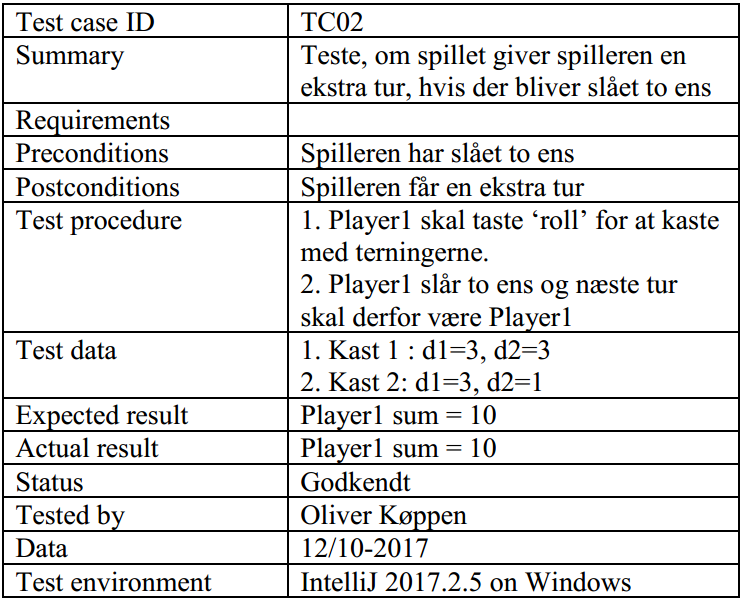
\includegraphics[width=10cm]{graphics/TC02}
    \end{center}
\end{figure}

Testcase 3 handler om, hvorvidt programmet husker det foregående kast, og om spilleren vinder, hvis personen slår to 6'ere på to kast.

\begin{figure}[h]
    \begin{center}
        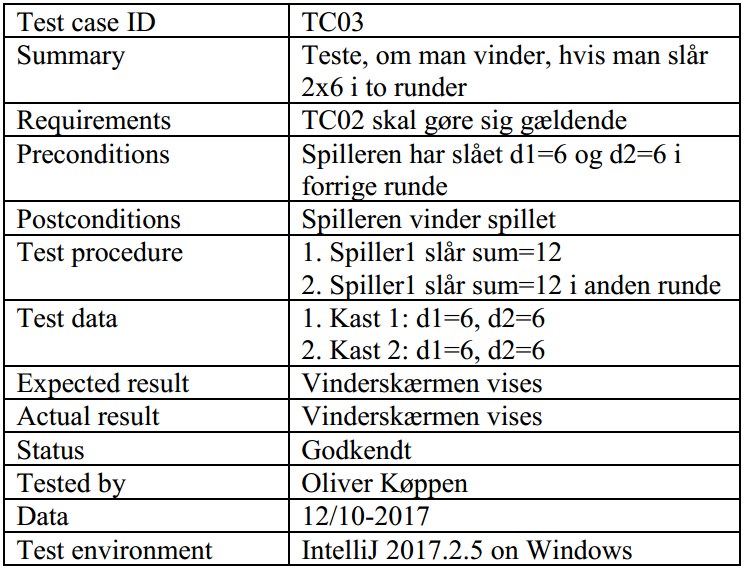
\includegraphics[width=10cm]{graphics/TC03}
    \end{center}
\end{figure}

Testcase 4 handler om, hvorvidt programmet resetter spillerens score, hvis personen slår to 1'ere.

\begin{figure}[h]
    \begin{center}
        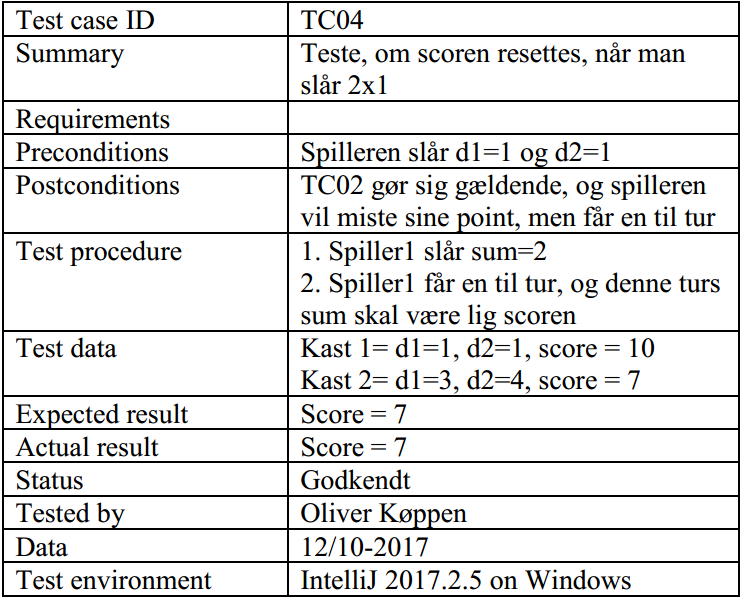
\includegraphics[width=10cm]{graphics/TC04}
    \end{center}
\end{figure}
\pagebreak

Testcase 5 handler om, at spilleren kun kan vinde, hvis personens score er større eller lig med 40, og der slås to ens.
\begin{figure}[h]
    \begin{center}
        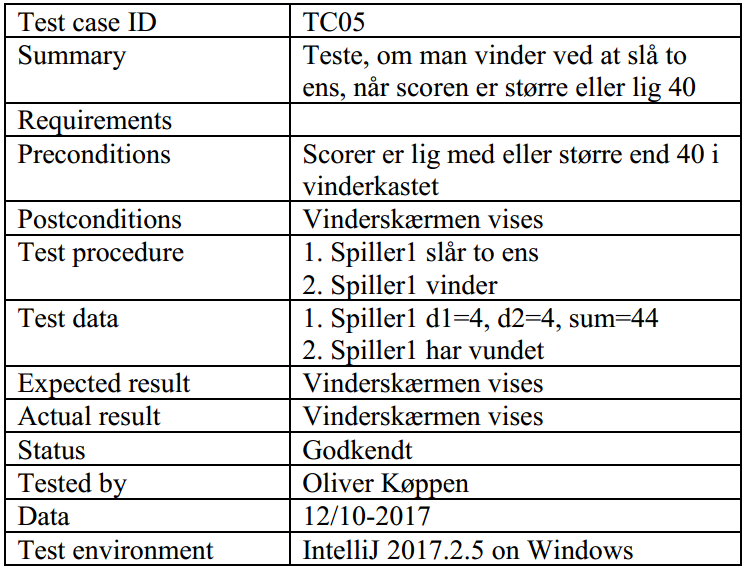
\includegraphics[width=10cm]{graphics/TC05}
    \end{center}
\end{figure}